	\subsection{Sposób filtracji}
Do danych zbieranych w projekcie często dojdą takie, które mogą zaburzyć otrzymanie prawidłowego wyniku. Jedną z metod, aby poradzić sobie z tym jest filtracja danych poprzez odrzucenie tych najbardziej skrajnych. Danych mozna odrzucić nawet połowę próbek, aczkolwiek przypadek przedstawiony tutaj nie potzrebuje aż tak rygorystycznych reguł. Dane, które odrzucimy to będą 3 próbki osób, które po prostu zawyżyły cenę swoich mieszkań. Ważnym jest, żeby przefiltrować dane w odpowiedni sposób odrzucając te próbki, które mogą mieć najbardziej negatywny wpływ na wynik końcowy.
	\subsection{Odrzucenie danych}
Skoro celem naszego algorytmu jest znalezienie zależności między ceną mieszkania, a jego metrażem, możemy stwierdzić w uproszczeniu, że poszukujemy tak naprawdę średniej ceny za metr kwadratowy mieszkania we Wrocławiu.
\newline
\newline
\noindent
\(
	y  \hspace{2.1cm} \textrm{cena mieszkania} [zl] \\
	X  \hspace{2cm} \textrm{powierzchnia mieszkania} [m^{2}] \\
	z = \frac{y}{X}  \hspace{1.3cm} \textrm{cena za metr kwadratowy} [\frac{zl}{m^{2}}] \\
\)


Najbardziej skrajne dane obliczamy za pomocą sumowania wszystkich 'z' oraz podzielenia tego przez liczbę próbek. W ten sposób znajdujemy średnią wartość kosztu za metr kwadratowy. Mozna sądzić, że w tym momencie mamy rozwiązany problem regresji liniowej, bo wystarczy skalować to na prostą. Po części tak, ale problemem tutaj nie jest samo znalezienie prostej, a opisanie jednej z metod pozyskiwania prostej opisującej jakieś dane.
\newline
\newline
\noindent
\(
	s  \hspace{2.1cm} \textrm{średnia cena za } m^{2} [zl] \\
	s = 6315,9 \\
	d_{i}  \hspace{2cm} \textrm{odchylenie od średniej } [zl] \\
	d_{i} = |s - z_{i}| \\
\)
W ten sposób otrzymamy \(d_{i}\) dla każdego elementu. Poszukujemy tych, których odchył jest największy. Według obliczeń są to odpowiednio pary:
\begin{itemize}

  \item 29.15 metrów za 294 000 zł
  \item 27 metrów za 259 000 zł
  \item 50 metrów za 477 000 zł

\end{itemize}

Dokładne zoobrazowanie tych danych jest przedstawione na poniższym wykresie 1D. 3 punkty stanowczo są odsunięte od średniej ceny za metr kwadratowej (niebieskie kółko).


	\begin{figure}[H]
    \centering
    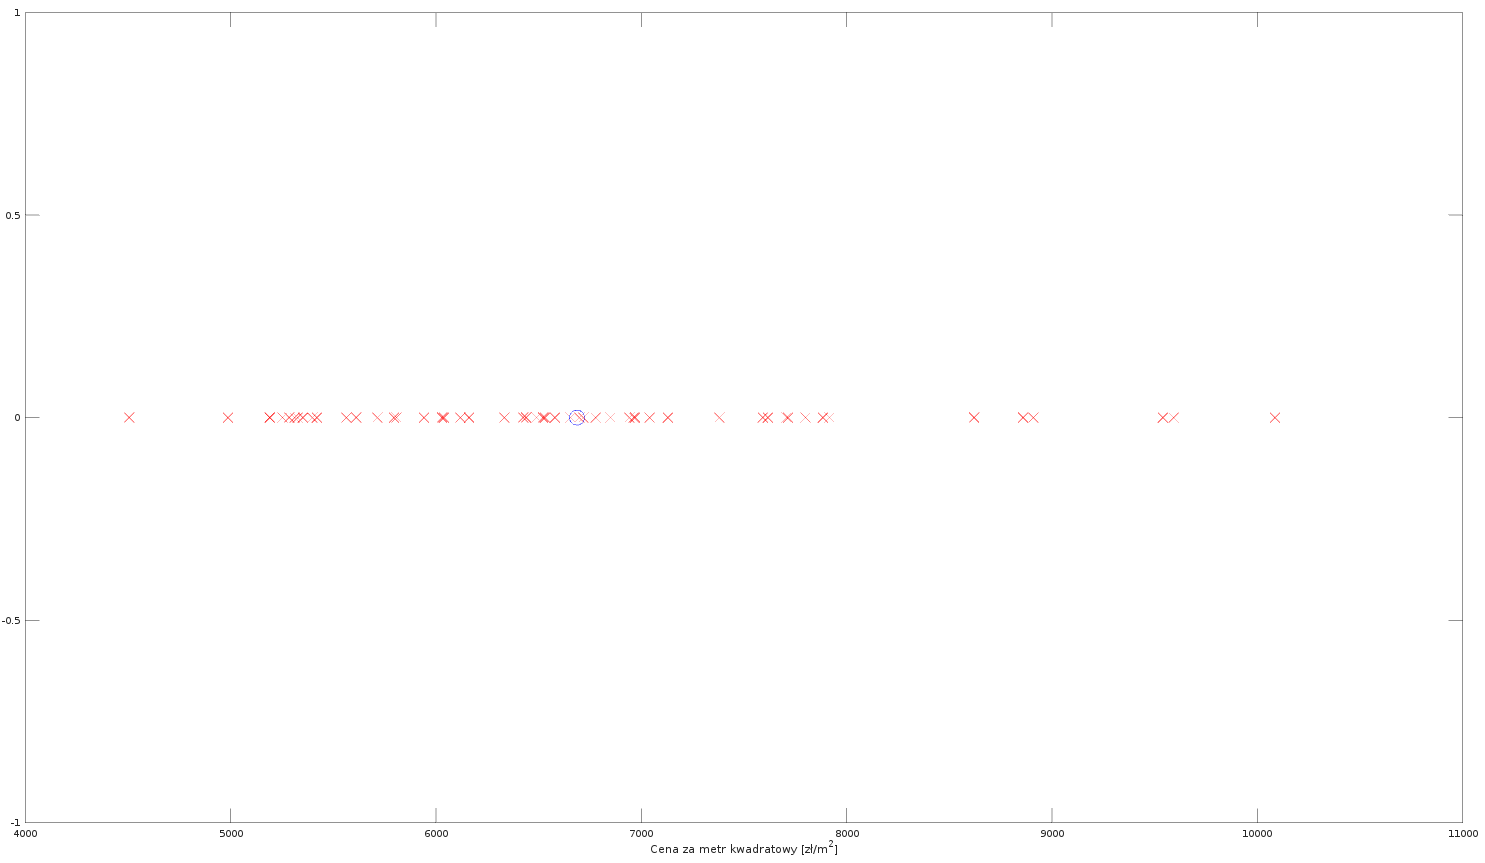
\includegraphics[scale=0.20]{PNG/1D.png}
    \caption{Wykres ceny metra kwadratowego dla wszystkich próbek}
    \label{lamana}
	\end{figure}
	

	\subsection{Dane po filtracji}
	- wykres danych po  \\
	- plusy filtracji \\
	- specyfika filtracji, inne punkty odrzucone niż na pierwszy rzuk oka \\